\documentclass[12pt]{article}

\usepackage[a4paper,margin=1in]{geometry}
\usepackage{amsmath,amssymb}
\usepackage{booktabs}
\usepackage{caption}
\usepackage{float}
\usepackage{graphicx}
\usepackage{hyperref}
\usepackage{setspace}
\usepackage{tikz}
\usetikzlibrary{arrows.meta,calc,decorations.pathreplacing,positioning}

\usepackage[
    backend=biber,
    style=numeric,
    sorting=none,
    maxcitenames=2,
    maxbibnames=99,
    giveninits=true
]{biblatex}

\addbibresource{qc_paper.bib}
\graphicspath{{../results/}{results/}}
\captionsetup{font=small}
\setstretch{1}
\setlength{\emergencystretch}{2em}

\title{\textbf{Quantum Amplitude Estimation for Option Pricing}}
\author{Jayneel Parikh}
\date{\today}

\begin{document}

\maketitle

\begin{abstract}
Quantum amplitude estimation promises a quadratic speedup over classical Monte Carlo for pricing financial derivatives, reducing the sample complexity from $O(\epsilon^{-2})$ to $O(\epsilon^{-1})$ for additive error~$\epsilon$.  This statement is a query-complexity result; it does not include variance reduction on the classical side or the cost of implementing the quantum oracle.  We test this distinction for European and arithmetic Asian call options.  The European case is used to validate the QAE pricing map with a statevector circuit.  The Asian case is used to compare simple Monte Carlo with the Kemna--Vorst control variate and to examine the circuit cost of path dependence through small finite-grid quantum oracles.  With daily monitoring, the control variate reduces the Asian standard error by a factor of $36.3$, so that $10^5$ variance-reduced paths have about the same variance as $1.32\times10^8$ plain paths.  A three-date toy Asian oracle already has depth $2396$ after transpilation, before amplitude estimation is applied.  These numbers do not locate a hardware crossover.  They identify which costs would have to enter that estimate.
\end{abstract}

\noindent{\itshape Note:} All figures are original and the source code is available at \url{https://github.com/jayneel-p}.


\section{Introduction}

A substantial portion of the computational resources deployed in financial markets is spent on pricing and risk management \cite{rebentrostQuantumComputationalFinance2018}.  Financial derivatives are contracts whose payoff depends on the future price or trajectory of an underlying asset.  Their prices require expectations under stochastic models, and only for simplest contracts do these expectations have a closed form.  The Black--Scholes--Merton model \cite{blackPricingOptionsCorporate1973,mertonTheoryRationalOption1973} prices vanilla European options analytically, but once the payoff depends on the path of the asset, or on several correlated assets, or if the underlying assumptions for the BS model fail (constant volatility, log-normal distribution, constant risk-free interest, perfect liquidity), the standard tool becomes Monte Carlo simulation \cite{glassermanMonteCarloMethods2004}.

Monte Carlo handles arbitrary payoff structures and stochastic dynamics with little change to the method.  Its cost is statistical: with $M$ independent paths the standard error decays as $O(M^{-1/2})$, so halving the error demands four times the computation.  This rate is a fundamental consequence of the central limit theorem, and it has motivated a long line of classical work aimed at reducing the variance of the estimator without changing the convergence exponent.  Kemna and Vorst \cite{kemnaPricingMethodOptions1990} observed that for arithmetic Asian options, whose payoff depends on the time-average of the underlying, the geometric-average Asian has a closed form and is highly correlated with the arithmetic payoff.  Using it as a control variate removes most of the sampling noise.  At daily monitoring frequency the standard error drops by a factor of roughly $36$, comparable to the $20\text{--}40\times$ range reported in the literature for similar regimes \cite{kemnaPricingMethodOptions1990,glassermanMonteCarloMethods2004}.  A quantum method for this contract should be compared with that reduced-variance scale, not only with simple Monte Carlo.

Quantum amplitude estimation \cite{brassardQuantumAmplitudeAmplification2002} tackles the same expectation-estimation problem from a different direction.  Given a unitary operator that prepares the probability distribution and encodes the payoff into an amplitude, amplitude estimation recovers the expectation with $O(\epsilon^{-1})$ oracle queries for additive error~$\epsilon$, a quadratic improvement over the classical sampling rate.  Rebentrost, Gupt, and Bromley \cite{rebentrostQuantumComputationalFinance2018} formulated this pricing map under the Black--Scholes model.  Stamatopoulos \textit{et al.}\ \cite{stamatopoulosOptionPricingUsing2020} made the construction explicit at the circuit level, including comparators, payoff rotations, weighted sums for basket and path-dependent options, and small IBM-hardware demonstrations.  Their reported full amplitude-estimation circuits for European examples already range from depth $3927$ at $m=3$ sampling qubits to depth $285204$ at $m=9$, before considering daily path dependence.  Wang and Kan \cite{wangOptionPricingStochastic2024} push the resource question further for Asian and barrier options under stochastic volatility: even their more efficient weak-Euler instances have $T$-counts of order $10^{11}$ and require $10^4$--$10^5$ logical qubits.  Manzano \textit{et al.}\ \cite{manzanoAlternativePipelineOption2025} study an alternative encoding pipeline, while Rendon \textit{et al.}\ \cite{rendonExponentialImprovementAsian2025} pursue a PDE-based route that changes the bottleneck rather than improving the same Monte Carlo estimator.

The QAE speedup should be read as a query-model statement.  It counts calls to the pricing oracle, not the cost of building that oracle.  Each oracle call is itself a quantum circuit whose depth grows with the number of qubits used to discretize the price distribution, the complexity of the payoff function, and the number of time steps in the path.  The classical baseline changes with the estimator.  For path-dependent and high-dimensional contracts, variance reduction can lower the effective cost of Monte Carlo by orders of magnitude.  Many existing quantum pricing papers benchmark against simple Monte Carlo, which can overstate the practical gap.

This paper separates three questions.  First, how much does the Kemna--Vorst control variate change the Asian Monte Carlo baseline?  Second, does the implemented European circuit encode the intended payoff expectation?  Third, how quickly does path dependence enter the oracle cost?  The answer is unfavorable to simple quantum-advantage narratives: the query speedup remains, but the classical baseline and the oracle are both stronger than the headline comparison suggests.

\section{Financial background}

\subsection{Risk-neutral geometric Brownian motion}

Let $S_t$ be the price of one risky asset at time $t$.  In the Black--Scholes model the physical-market dynamics are written
\begin{equation}
    dS_t = \mu S_t\,dt + \sigma S_t\,dW_t,
\end{equation}
where $\mu$ is the physical drift, $\sigma>0$ is the volatility, and $W_t$ is a Brownian motion.  Pricing is performed under a risk-neutral measure $\mathbb{Q}$, where the drift is the risk-free rate $r$.  The pricing dynamics are
\begin{equation}
    dS_t = rS_t\,dt + \sigma S_t\,dW_t^{\mathbb{Q}}.
    \label{eq:risk-neutral-gbm}
\end{equation}
Here $W_t^{\mathbb{Q}}$ is Brownian motion under $\mathbb{Q}$.  This is the model used in the simulations below and in the standard quantum-pricing setup \cite{rebentrostQuantumComputationalFinance2018,stamatopoulosOptionPricingUsing2020}.

For initial asset price $S_0$ and maturity time $T$, Eq.~\eqref{eq:risk-neutral-gbm} gives
\begin{equation}
    S_T = S_0
    \exp\!\left[
        \left(r-\frac{1}{2}\sigma^2\right)T
        + \sigma\sqrt{T}\,Z
    \right],
    \qquad Z\sim N(0,1).
    \label{eq:gbm-solution}
\end{equation}
where $Z$ is a standard normal random variable.  Thus $S_T$ is lognormal.

\begin{figure}[H]
    \centering
    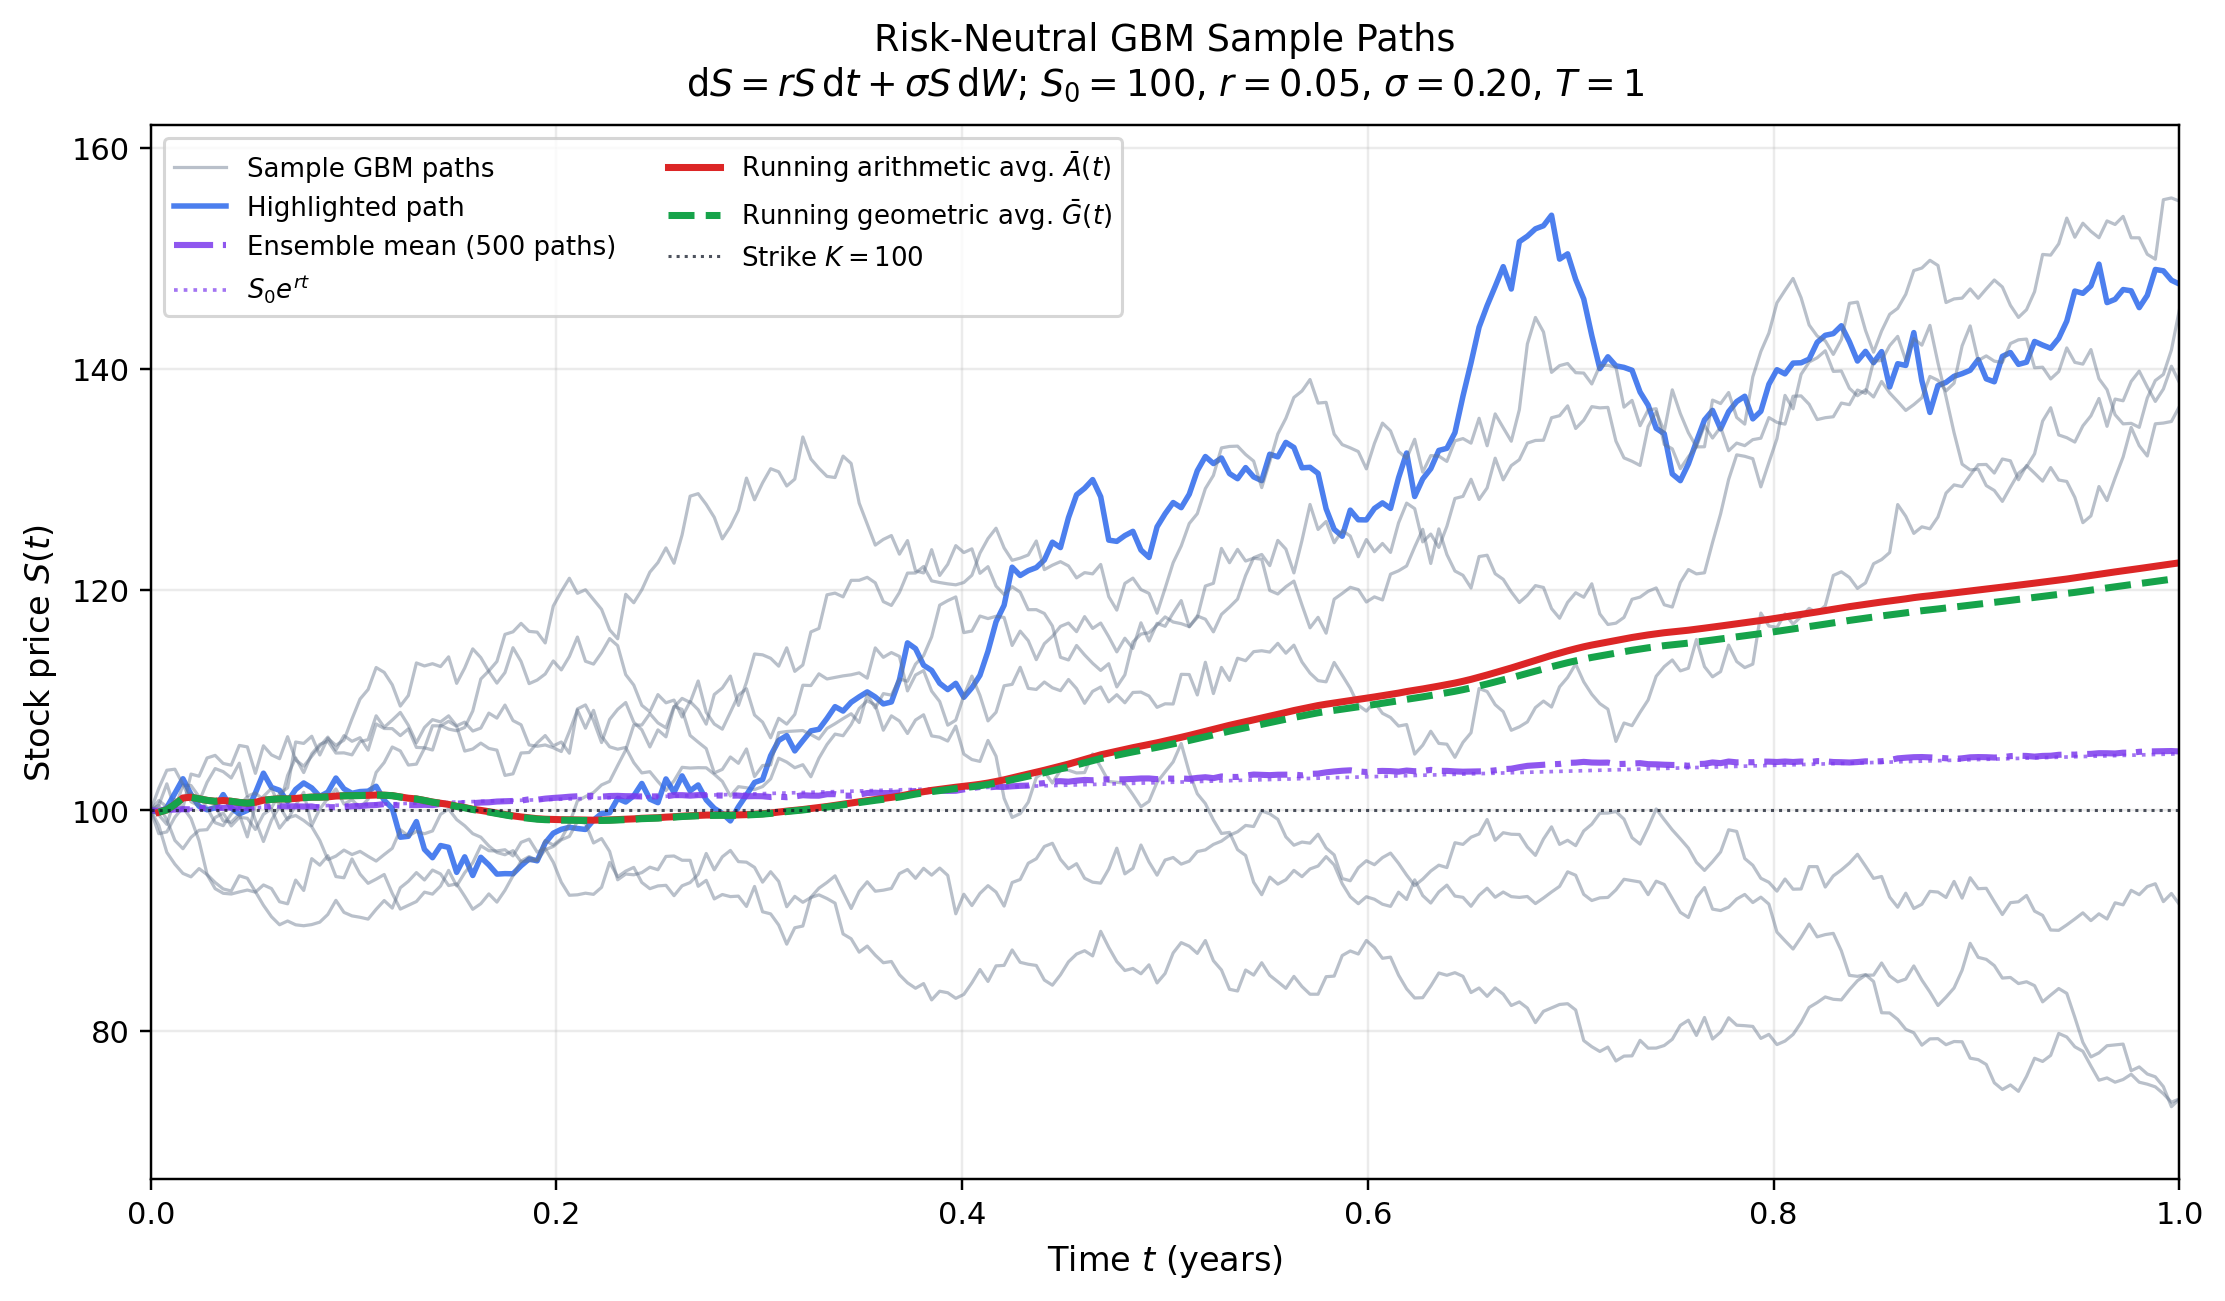
\includegraphics[width=0.74\textwidth]{gbm_sample_paths.png}
    \caption{Sample geometric Brownian motion paths under the risk-neutral model.  European payoffs depend only on $S_T$, while Asian payoffs depend on the path average.}
    \label{fig:gbm-paths}
\end{figure}

If $f$ is the payoff paid at time $T$, the time-zero price is
\begin{equation}
    V_0 = e^{-rT}\mathbb{E}_{\mathbb{Q}}\!\left[f\right].
    \label{eq:risk-neutral-price}
\end{equation}
Here $V_0$ is the option value at time zero and $e^{-rT}$ is the discount factor.

\subsection{European calls}

A European call with strike $K$ has payoff
\begin{equation}
    f_{\mathrm{E}}(S_T)=\max(S_T-K,0).
\end{equation}
Here $f_{\mathrm{E}}$ denotes the European-call payoff and $S_T$ is the terminal asset price.  Under Eq.~\eqref{eq:risk-neutral-gbm}, its Black--Scholes price is
\begin{equation}
    C_{\mathrm{BS}}
    = S_0\Phi(d_1)-Ke^{-rT}\Phi(d_2),
    \label{eq:black-scholes}
\end{equation}
where $C_{\mathrm{BS}}$ is the Black--Scholes call price, $\Phi$ is the standard normal cumulative distribution function, and
\begin{align}
    d_1 &=
    \frac{\log(S_0/K)+(r+\frac{1}{2}\sigma^2)T}
         {\sigma\sqrt{T}},
    &
    d_2 &= d_1-\sigma\sqrt{T}.
\end{align}
The quantities $d_1$ and $d_2$ are the normalized log-moneyness terms.  This closed form is used as a benchmark.

\subsection{Arithmetic Asian calls}

Let $t_1,\ldots,t_N$ be $N$ monitoring dates satisfying
\begin{equation}
    0<t_1<t_2<\cdots<t_N=T.
\end{equation}
The arithmetic Asian call depends on the average of the asset prices at these dates.  The dates are taken equally spaced and $S_0$ is not included.  The arithmetic average is
\begin{equation}
    A_N = \frac{1}{N}\sum_{i=1}^{N}S_{t_i},
\end{equation}
where $A_N$ is the average over the monitored prices.  The payoff is
\begin{equation}
    f_{\mathrm{A}} = \max(A_N-K,0).
    \label{eq:arith-asian-payoff}
\end{equation}
Here $f_{\mathrm{A}}$ denotes the arithmetic Asian payoff.  The arithmetic average of lognormal random variables is not lognormal, so Eq.~\eqref{eq:arith-asian-payoff} has no Black--Scholes-type closed form in this model.

The corresponding geometric average is
\begin{equation}
    G_N =
    \left(\prod_{i=1}^{N}S_{t_i}\right)^{1/N}
    =
    \exp\!\left(\frac{1}{N}\sum_{i=1}^{N}\log S_{t_i}\right).
\end{equation}
Here $G_N$ is the geometric average over the same monitoring dates.  Since the log-prices are jointly normal, $\log G_N$ is normal.  The geometric Asian call therefore has a closed-form price and is highly correlated with the arithmetic Asian call.  Kemna and Vorst use this structure as a control variate \cite{kemnaPricingMethodOptions1990}.

For equally spaced fixings excluding $S_0$, define the effective geometric volatility $\sigma_G$ and drift parameter $m_G$ by
\begin{equation}
    \sigma_G
    =
    \sigma
    \sqrt{
        \frac{(N+1)(2N+1)}{6N^2}
    },
    \qquad
    m_G =
    \left(r-\frac{1}{2}\sigma^2\right)\frac{N+1}{2N}.
    \label{eq:geo-params}
\end{equation}
Then the logarithm of the geometric average is distributed as
\begin{equation}
    \log G_N
    \sim
    N\!\left(
        \log S_0 + m_GT,\,
        \sigma_G^2T
    \right).
\end{equation}
The resulting geometric Asian call price is
\begin{equation}
    C_G
    =
    e^{-rT}
    \left[
        S_0e^{(m_G+\frac{1}{2}\sigma_G^2)T}\Phi(\widetilde d_1)
        -
        K\Phi(\widetilde d_2)
    \right],
    \label{eq:geo-asian-price}
\end{equation}
where $C_G$ is the geometric Asian call price and
\begin{align}
    \widetilde d_1
    &=
    \frac{\log(S_0/K)+(m_G+\sigma_G^2)T}
         {\sigma_G\sqrt{T}},
    &
    \widetilde d_2
    &=
    \widetilde d_1-\sigma_G\sqrt{T}.
\end{align}
The variables $\widetilde d_1$ and $\widetilde d_2$ are the analogues of $d_1$ and $d_2$ for the distribution of $G_N$.

\section{Classical Monte Carlo baseline}

\subsection{Simple Monte Carlo}

Let $X$ be the discounted payoff
\begin{equation}
    X = e^{-rT}f
\end{equation}
where $f$ is the payoff at maturity.  If $X_1,\ldots,X_M$ are independent samples of $X$, the simple Monte Carlo estimator is
\begin{equation}
    \widehat V_M
    =
    \frac{1}{M}\sum_{j=1}^{M}X_j.
    \label{eq:mc-estimator}
\end{equation}
where $\widehat V_M$ is the estimated time-zero price.  The estimator is unbiased under the risk-neutral model.  Its standard error is
\begin{equation}
    \mathrm{SE}(\widehat V_M)
    =
    \frac{\sqrt{\mathrm{Var}(X)}}{\sqrt{M}},
    \label{eq:mc-se}
\end{equation}
where $\mathrm{Var}(X)$ is the payoff variance.  In computation this is estimated by replacing $\mathrm{Var}(X)$ with the sample variance.  The $M^{-1/2}$ dependence is the classical Monte Carlo rate \cite{stamatopoulosOptionPricingUsing2020,xuPricingArithmeticAverage2023}.

For the European call, samples are drawn directly from Eq.~\eqref{eq:gbm-solution}.  For the arithmetic Asian call, paths are simulated on the monitoring grid.  With time step $\Delta t=T/N$, the exact geometric Brownian transition is
\begin{equation}
    S_{t_{i+1}}
    =
    S_{t_i}
    \exp\!\left[
        \left(r-\frac{1}{2}\sigma^2\right)\Delta t
        + \sigma\sqrt{\Delta t}\,Z_i
    \right],
    \qquad Z_i\sim N(0,1).
    \label{eq:gbm-step}
\end{equation}
Here $S_{t_i}$ and $S_{t_{i+1}}$ are consecutive monitored prices and $Z_i$ is a standard normal draw.  The grid values are therefore sampled without time-discretization bias.

The numerical experiments use the parameter set
\begin{equation}
    S_0=100,\qquad K=100,\qquad r=0.05,\qquad \sigma=0.2,\qquad T=1.
\end{equation}
For the Asian option, $N=252$ daily monitoring dates are used.  The European Black--Scholes benchmark is
\begin{equation}
    C_{\mathrm{BS}}=10.450584.
\end{equation}
The geometric Asian benchmark is
\begin{equation}
    C_G=5.565509.
\end{equation}

\subsection{Kemna--Vorst control variate}

Simple Monte Carlo is not the strongest classical baseline for Asian options.  Let
\begin{equation}
    X = e^{-rT}\max(A_N-K,0)
\end{equation}
be the discounted arithmetic payoff and let
\begin{equation}
    Y = e^{-rT}\max(G_N-K,0)
\end{equation}
be the discounted geometric payoff.  Here $X$ is the target payoff and $Y$ is the control payoff.  The expectation $\theta=\mathbb{E}[Y]$ is known from Eq.~\eqref{eq:geo-asian-price}.  A control-variate estimator is
\begin{equation}
    \widehat V_{\mathrm{CV}}
    =
    \overline X
    +
    \widehat\beta
    \left(\theta-\overline Y\right),
    \label{eq:cv-estimator}
\end{equation}
where $\overline X$ and $\overline Y$ are sample averages over the same simulated paths and
\begin{equation}
    \widehat\beta
    =
    \frac{\widehat{\mathrm{Cov}}(X,Y)}
         {\widehat{\mathrm{Var}}(Y)}.
    \label{eq:cv-beta}
\end{equation}
The quantity $\widehat\beta$ estimates the variance-minimizing coefficient $\beta^\ast=\mathrm{Cov}(X,Y)/\mathrm{Var}(Y)$.  The estimator remains centered on the arithmetic Asian price but removes the part of the arithmetic payoff fluctuation explained by the geometric payoff.

For $M=100{,}000$ paths and $N=252$ fixings, the plain estimator has standard error $0.025301$.  The Kemna--Vorst estimator has standard error $0.000697$.  This is a standard-error reduction of $36.3$ and a variance reduction of $1.32\times 10^3$.  In this parameter regime, $10^5$ control-variate paths have about the same variance as $1.32\times 10^8$ simple Monte Carlo paths.

\begin{figure}[H]
    \centering
    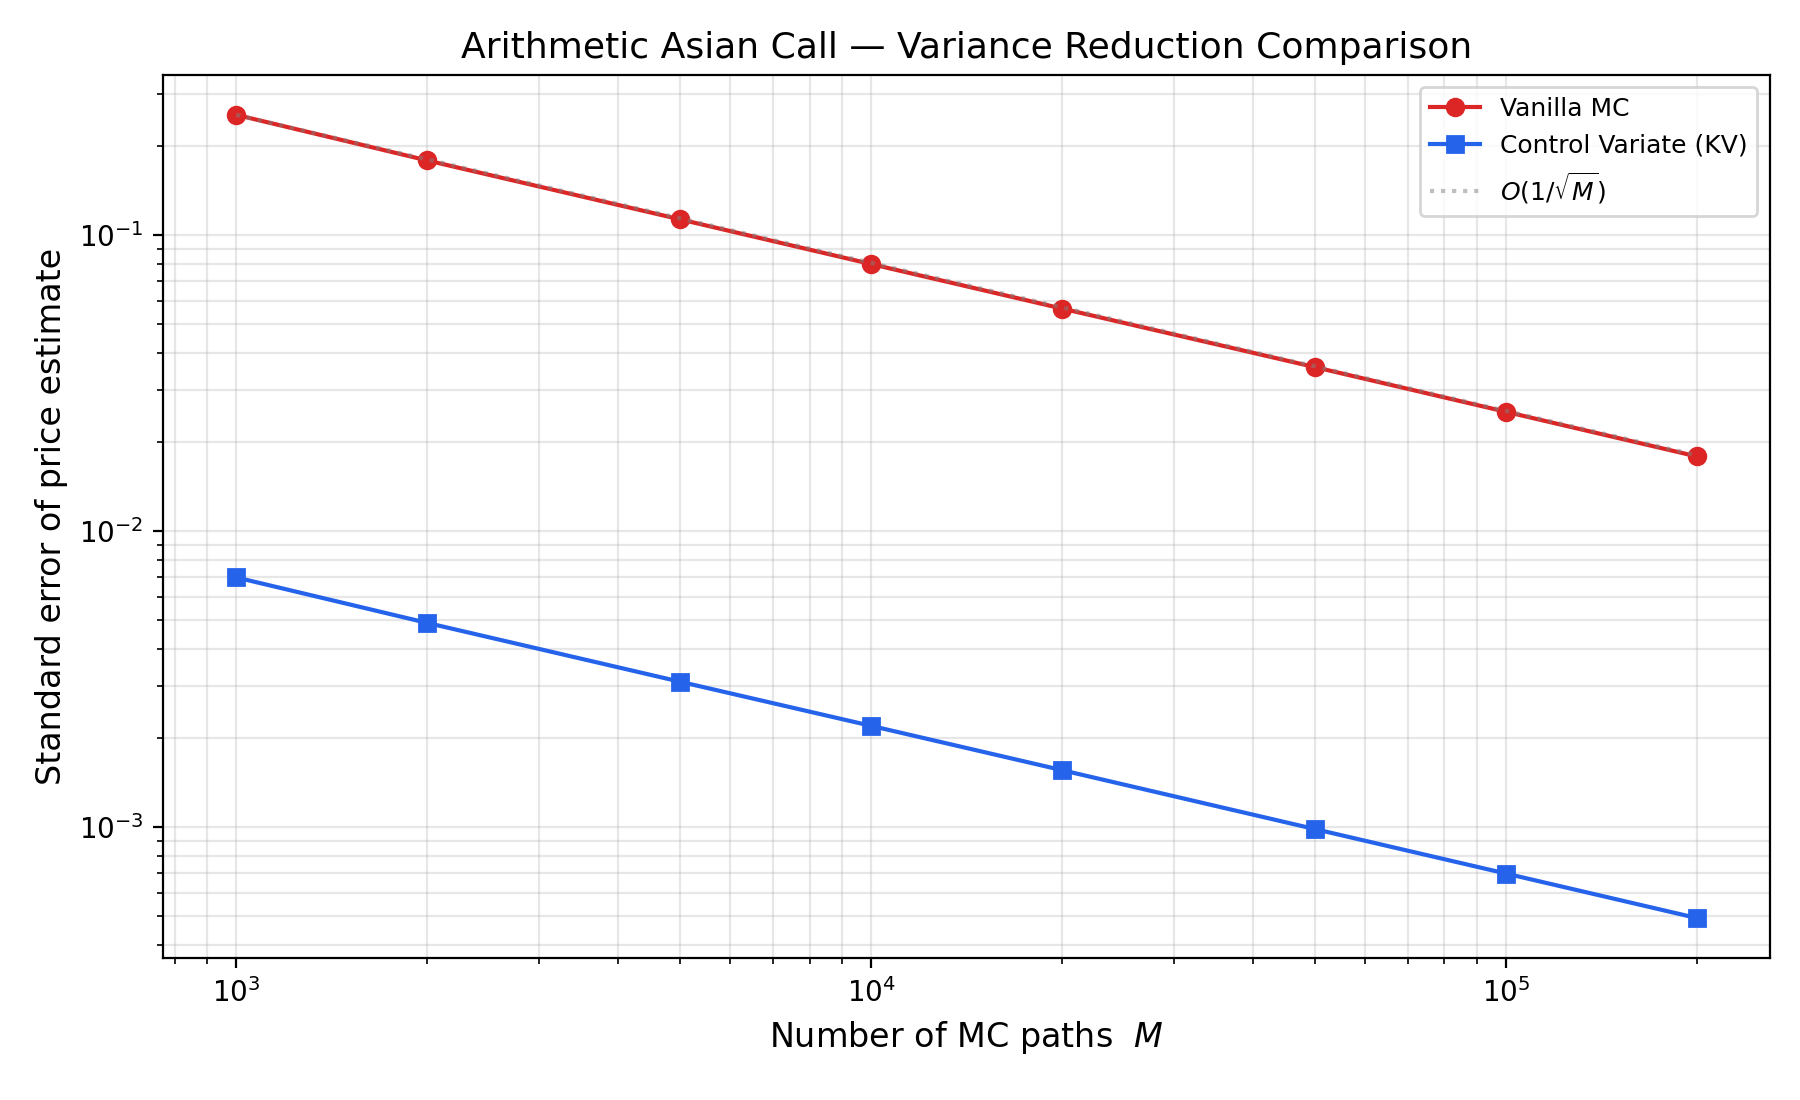
\includegraphics[width=0.74\textwidth]{asian_methods_comparison.png}
    \caption{Standard error for the arithmetic Asian call using simple Monte Carlo and the Kemna--Vorst control variate.  Both estimators use the same simulated paths in each trial.}
    \label{fig:asian-comparison}
\end{figure}

The control variate leaves the $M^{-1/2}$ rate in place, but it lowers the constant by a large factor.  This is the baseline used below.

\section{Quantum amplitude estimation framework}

\subsection{Encoding an expectation as an amplitude}

The quantum approach does not sample payoffs.  Instead it encodes the undiscounted payoff expectation as the probability of measuring a single qubit in the state $\lvert 1\rangle$.  Discounting by $e^{-rT}$ is applied classically afterward, exactly as in Eq.~\eqref{eq:risk-neutral-price}.

Discretize the terminal asset price onto $2^n$ grid points $x_0,\ldots,x_{2^n-1}$ with probabilities $p_i = \Pr[X=x_i]$.  A distribution-loading unitary $P_X$ prepares the state
\begin{equation}
    P_X\lvert 0\rangle_n
    =
    \sum_{i=0}^{2^n-1}\sqrt{p_i}\,\lvert i\rangle_n ,
    \label{eq:distribution-loading}
\end{equation}
where $\lvert i\rangle_n$ is the $n$-qubit computational basis state representing $x_i$.  The amplitudes are square roots of probabilities, so that the Born rule returns $p_i$ upon measurement of basis state $\lvert i\rangle$.  The price register, any ancillas, and the objective qubit are part of one joint quantum state.  Payoff operations may entangle these registers, but the full map remains unitary until the final measurement.

\begin{figure}[H]
    \centering
    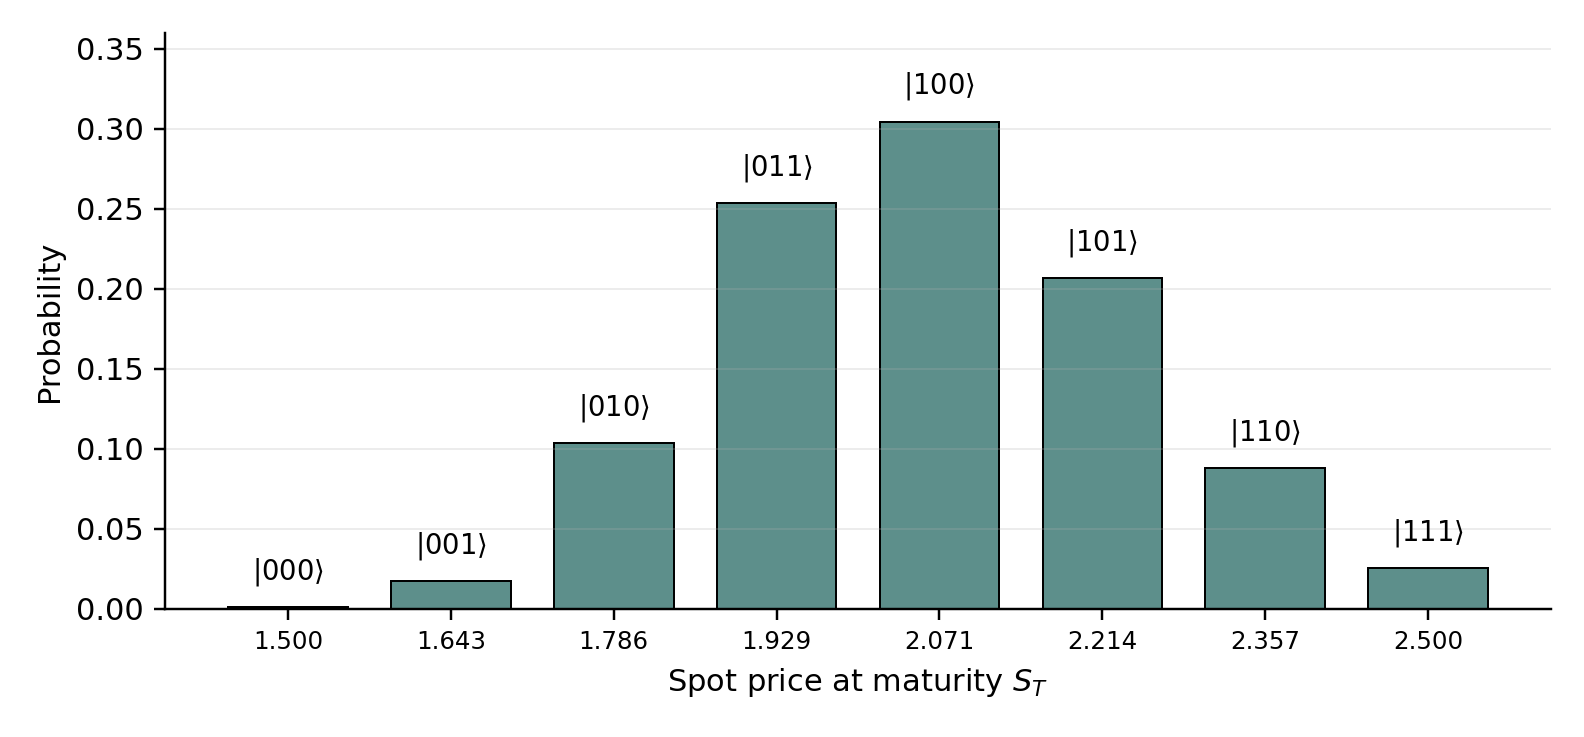
\includegraphics[width=0.82\textwidth]{stamatopoulos_fig3_reproduction.png}
    \caption{Reproduction of the three-qubit log-normal maturity distribution used in Fig.~3 of Stamatopoulos \textit{et al.}\ \cite{stamatopoulosOptionPricingUsing2020}.  The basis labels are the states loaded by $P_X$.  Parameters: $S_0=2$, $r=0.04$, $\sigma=0.10$, $T=300/365$, and $S_T\in[1.5,2.5]$.}
    \label{fig:stamatopoulos-fig3}
\end{figure}

Let $g_i=g(x_i)$ be the payoff at grid point $x_i$, and let $g_{\max}$ bound it from above so that the normalized payoff $f_i = g_i/g_{\max}$ satisfies $0\le f_i\le 1$.  A payoff unitary $U_f$ rotates one objective qubit conditioned on the price register:
\begin{equation}
    U_f\lvert i\rangle_n\lvert 0\rangle
    =
    \lvert i\rangle_n
    \left(
        \sqrt{1-f_i}\,\lvert 0\rangle
        +
        \sqrt{f_i}\,\lvert 1\rangle
    \right).
    \label{eq:payoff-loading}
\end{equation}
The full state-preparation operator $A = U_f(P_X\otimes I)$ acts on $n+1$ qubits.  Applying it to the all-zero input gives
\begin{equation}
    A\lvert 0\rangle_n\lvert 0\rangle
    =
    \sqrt{1-a}\,\lvert \psi_0\rangle
    +
    \sqrt{a}\,\lvert \psi_1\rangle,
    \label{eq:a-good-bad}
\end{equation}
where $\lvert \psi_1\rangle$ collects all terms with objective qubit $\lvert 1\rangle$ and $\lvert \psi_0\rangle$ collects those with $\lvert 0\rangle$.  The Born rule now does the work.  The probability of measuring the objective qubit in state $\lvert 1\rangle$ is the sum of the squared amplitudes in the $\lvert 1\rangle$ subspace, which by construction equals
\begin{equation}
    a
    =
    \Pr[\text{objective}=1]
    =
    \sum_{i=0}^{2^n-1} p_i f_i
    =
    \mathbb{E}[f(X)].
    \label{eq:amplitude-expectation}
\end{equation}
Thus the measurement probability is exactly the normalized expected payoff.  The operator $A$ follows the prepare-then-compute pattern common to quantum algorithms.  Here $P_X$ prepares the input distribution, $U_f$ computes the function of interest into an ancilla amplitude, and measurement extracts the expectation \cite{rebentrostQuantumComputationalFinance2018,stamatopoulosOptionPricingUsing2020}.

For a European call, $g_i=\max(x_i-K,0)$ and the time-zero price is
\begin{equation}
    C_0 = e^{-rT}g_{\max}\,a.
    \label{eq:european-amplitude-price}
\end{equation}
Stamatopoulos \textit{et al.}\ implement $U_f$ with controlled $R_y$ rotations and a first-order approximation to the payoff map \cite{stamatopoulosOptionPricingUsing2020}.  The implementation used here keeps the same division between distribution loading and payoff rotation.

\subsection{Amplitude amplification and estimation}

Estimating $a$ by repeated measurement of $A\lvert 0\rangle_n\lvert 0\rangle$ would reproduce the $O(M^{-1/2})$ Monte Carlo rate.  The quadratic improvement comes from amplitude estimation, which repeatedly applies the Grover iterate defined below \cite{brassardQuantumAmplitudeAmplification2002}.  In Grover search the goal is to find a marked item; here the ``marked'' states are those where the option finishes in the money, and the goal is to estimate their total weight.

Define the projector $\Pi_1 = I_n\otimes \lvert 1\rangle\langle 1\rvert$ onto the subspace where the objective qubit is $\lvert 1\rangle$, and the two reflections
\begin{equation}
    S_1 = I - 2\Pi_1,
    \qquad
    S_0 = I - 2\lvert 0\rangle_{n+1}\langle 0\rvert_{n+1}.
\end{equation}
The Grover iterate is
\begin{equation}
    Q = - A S_0 A^\dagger S_1.
    \label{eq:grover-iterate}
\end{equation}
The reflection $S_1$ marks the good subspace; $A S_0 A^\dagger$ reflects about the prepared state.  Two reflections compose into a rotation in the two-dimensional subspace spanned by $\lvert\psi_0\rangle$ and $\lvert\psi_1\rangle$.  Writing $a=\sin^2\theta$ with $\theta\in[0,\pi/2]$, repeated applications give
\begin{equation}
    Q^k A\lvert 0\rangle_n\lvert 0\rangle
    =
    \cos\!\left((2k+1)\theta\right)\lvert \psi_0\rangle
    +
    \sin\!\left((2k+1)\theta\right)\lvert \psi_1\rangle,
    \label{eq:grover-rotation}
\end{equation}
Hence each application of $Q$ advances the state by angle $2\theta$ toward the good subspace.  Amplitude estimation recovers $\theta$, and hence $a=\sin^2\theta$, by applying phase estimation to $Q$ \cite{brassardQuantumAmplitudeAmplification2002}.  With $M=2^m$ oracle calls the error scales as $O(M^{-1})$, the quadratic improvement over sampling.

The numerical experiments use iterative amplitude estimation (IAE), which avoids the inverse quantum Fourier transform and controlled-$Q^{2^j}$ powers of the circuit.  IAE estimates the same angle $\theta$ through a sequence of Grover iterates at different depths, combined with classical likelihood inference \cite{grinkoIterativeQuantumAmplitude2021,stamatopoulosOptionPricingUsing2020}.  At each depth $k$, the measured success probability is $\sin^2((2k+1)\theta)$, so the classical post-processing updates an interval for $\theta$ rather than reading it from a phase-estimation register.  Only the estimation subroutine differs from canonical QAE; the state preparation in Eqs.~\eqref{eq:distribution-loading}--\eqref{eq:amplitude-expectation} is unchanged.

\subsection{European-call circuit}

The operator $A$ for a European call has two stages: $i)$ load the terminal price distribution and $ii)$ rotate the objective qubit according to the normalized payoff.  Fig.~\ref{fig:a-operator-circuit} shows the high-level structure.  In practice, $a$ is estimated by IAE rather than by naive Bernoulli sampling of the objective qubit; the classical rescaling in Eq.~\eqref{eq:european-amplitude-price} then recovers the option price \cite{grinkoIterativeQuantumAmplitude2021,stamatopoulosOptionPricingUsing2020}.

\begin{figure}[H]
    \centering
    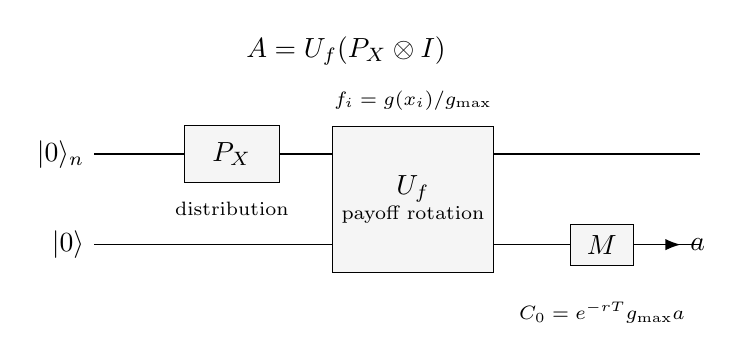
\begin{tikzpicture}[
        x=1cm,
        y=1cm,
        wire/.style={line width=0.55pt},
        gate/.style={draw, fill=gray!8, minimum height=0.72cm, align=center},
        smallgate/.style={draw, fill=gray!8, minimum height=0.52cm, align=center},
        >=Latex
    ]
        \coordinate (p0) at (0,1.7);
        \coordinate (q0) at (0,0.55);
        \draw[wire] (p0) -- (7.7,1.7);
        \draw[wire] (q0) -- (7.7,0.55);
        \node[left] at (p0) {$\lvert 0\rangle_n$};
        \node[left] at (q0) {$\lvert 0\rangle$};
        \node[gate, minimum width=1.2cm] (px) at (1.75,1.7) {$P_X$};
        \node[below=0.12cm of px] {\scriptsize distribution};

        \node[gate, minimum width=2.05cm, minimum height=1.85cm] (uf) at (4.05,1.125) {$U_f$\\[-1mm]\scriptsize payoff rotation};
        \node[above=0.08cm of uf] {\scriptsize $f_i=g(x_i)/g_{\max}$};

        \node[smallgate, minimum width=0.8cm] (m) at (6.45,0.55) {$M$};
        \draw[->, wire] (6.85,0.55) -- (7.45,0.55);
        \node[right] at (7.45,0.55) {$a$};

        \node[above] at (3.2,2.7) {$A=U_f(P_X\otimes I)$};
        \node[below] at (6.45,-0.05) {\scriptsize $C_0=e^{-rT}g_{\max}a$};
    \end{tikzpicture}
    \caption{State-preparation circuit for a European call.  The distribution loader $P_X$ prepares the discretized law of $S_T$, and $U_f$ rotates the objective qubit by an amount determined by the normalized payoff.}
    \label{fig:a-operator-circuit}
\end{figure}

The circuits below follow the gate-level decomposition of Stamatopoulos \textit{et al.}\ and are meant to make the oracle structure explicit.  Our implementation uses Qiskit Finance's log-normal distribution loader and \texttt{LinearAmplitudeFunction} to produce the same normalized piecewise-linear payoff rotation \cite{qiskitFinanceSoftware}.  Thus the code and the figures implement the same pricing map, although our code delegates the low-level comparator and rotation to Qiskit rather than the gates shown here. 

Stamatopoulos \textit{et al.}\ implement $U_f$ in two stages \cite{stamatopoulosOptionPricingUsing2020}. A reversible comparator determines whether the encoded price index $i$ exceeds the strike.  Let $t[k]$ be the $k$th bit of the strike in binary.  The comparator acts on the price register $\lvert i\rangle_n$, carry ancillas $\lvert a_1\rangle,\ldots,\lvert a_n\rangle$, and a comparator qubit $\lvert c\rangle$, setting $\lvert c\rangle=\lvert 1\rangle$ when $i\ge K$.  The construction uses only CNOT and Toffoli gates, similar to the half-adder.

\begin{figure}[H]
    \centering
    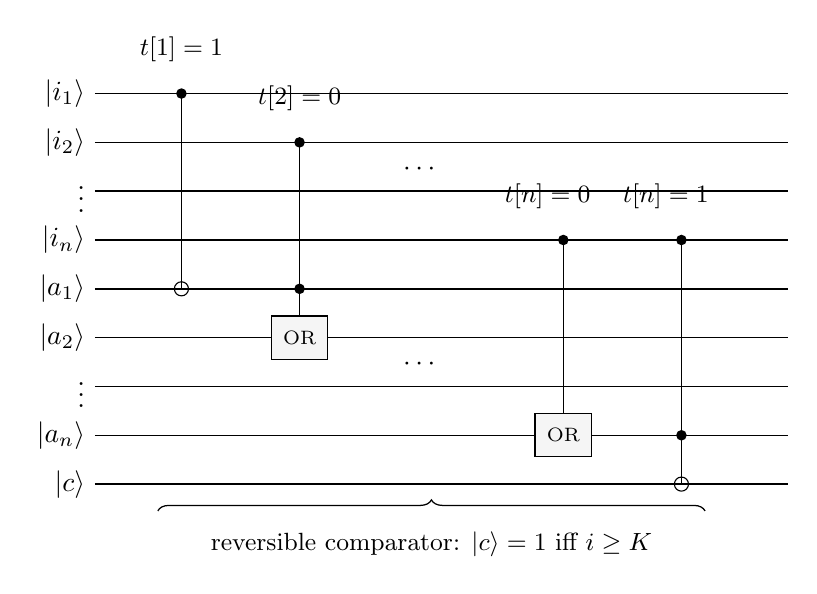
\begin{tikzpicture}[
        x=1cm,
        y=0.62cm,
        wire/.style={line width=0.5pt},
        gate/.style={draw, fill=gray!8, minimum height=0.55cm, align=center},
        dot/.style={circle, fill=black, inner sep=1.35pt},
        target/.style={circle, draw, inner sep=1.8pt},
        >=Latex
    ]
        \foreach \y/\lab in {
            8/{\lvert i_1\rangle},
            7/{\lvert i_2\rangle},
            6/{\vdots},
            5/{\lvert i_n\rangle},
            4/{\lvert a_1\rangle},
            3/{\lvert a_2\rangle},
            2/{\vdots},
            1/{\lvert a_n\rangle},
            0/{\lvert c\rangle}
        }{
            \draw[wire] (0,\y) -- (8.8,\y);
            \node[left] at (0,\y) {$\lab$};
        }

        \node[above] at (1.1,8.45) {\small $t[1]=1$};
        \node[dot] at (1.1,8) {};
        \draw[wire] (1.1,8) -- (1.1,4);
        \node[target] at (1.1,4) {};

        \node[above] at (2.6,7.45) {\small $t[2]=0$};
        \node[dot] at (2.6,7) {};
        \node[dot] at (2.6,4) {};
        \draw[wire] (2.6,7) -- (2.6,3);
        \node[gate, minimum width=0.72cm] at (2.6,3) {\scriptsize OR};

        \node at (4.15,6.45) {$\cdots$};
        \node at (4.15,2.45) {$\cdots$};

        \node[above] at (5.75,5.45) {\small $t[n]=0$};
        \node[dot] at (5.95,5) {};
        \node[dot] at (5.95,1) {};
        \draw[wire] (5.95,5) -- (5.95,1);
        \node[gate, minimum width=0.72cm] at (5.95,1) {\scriptsize OR};

        \node[above] at (7.25,5.45) {\small $t[n]=1$};
        \node[dot] at (7.45,5) {};
        \node[dot] at (7.45,1) {};
        \draw[wire] (7.45,5) -- (7.45,0);
        \node[target] at (7.45,0) {};

        \draw[decorate, decoration={brace, amplitude=4pt}, line width=0.45pt]
            (0.8,-0.55) -- (7.75,-0.55)
            node[midway, below=4pt] {\small reversible comparator: $\lvert c\rangle=1$ iff $i\ge K$};
    \end{tikzpicture}
    \caption{Comparator structure used for the European call, following the construction of Stamatopoulos \textit{et al.}\ \cite{stamatopoulosOptionPricingUsing2020}.  Only one of the $t[k]=0$ or $t[k]=1$ branches is used for each bit of the fixed strike.}
    \label{fig:comparator-circuit}
\end{figure}

The OR gate in Fig.~\ref{fig:comparator-circuit} decomposes into Pauli-$X$ gates and a Toffoli, as shown in Fig.~\ref{fig:or-gate}: negate the inputs, apply a Toffoli (which computes AND), negate the output and restore the inputs.  The result is $c \leftarrow a \lor b$ with $a$ and $b$ unchanged.

\begin{figure}[H]
    \centering
    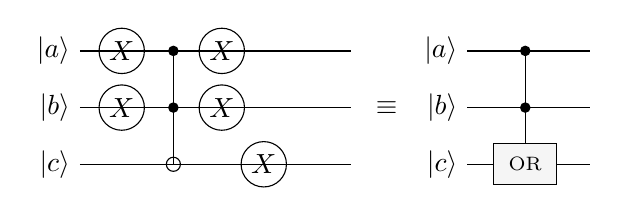
\begin{tikzpicture}[
        x=0.82cm,
        y=0.72cm,
        wire/.style={line width=0.5pt},
        xgate/.style={draw, circle, inner sep=1.8pt},
        dot/.style={circle, fill=black, inner sep=1.35pt},
        target/.style={circle, draw, inner sep=1.8pt},
        gate/.style={draw, fill=gray!8, minimum width=0.8cm, minimum height=0.52cm, align=center}
    ]
        \foreach \y/\lab in {2/{\lvert a\rangle},1/{\lvert b\rangle},0/{\lvert c\rangle}}{
            \draw[wire] (0,\y) -- (4.2,\y);
            \node[left] at (0,\y) {$\lab$};
        }
        \foreach \x in {0.65,2.2}{
            \node[xgate] at (\x,2) {$X$};
            \node[xgate] at (\x,1) {$X$};
        }
        \node[dot] at (1.45,2) {};
        \node[dot] at (1.45,1) {};
        \draw[wire] (1.45,2) -- (1.45,0);
        \node[target] at (1.45,0) {};
        \node[xgate] at (2.85,0) {$X$};

        \node at (5.18,1) {$\equiv \ \ \ \ \ \ $} ;

        \foreach \y/\lab in {2/{\lvert a\rangle},1/{\lvert b\rangle},0/{\lvert c\rangle}}{
            \draw[wire] (6.0,\y) -- (7.9,\y);
            \node[left] at (6.0,\y) {$\lab$};
        }
        \node[dot] at (6.9,2) {};
        \node[dot] at (6.9,1) {};
        \draw[wire] (6.9,2) -- (6.9,0);
        \node[gate] at (6.9,0) {\scriptsize OR};
    \end{tikzpicture}
    \caption{Reversible OR subcircuit used inside the comparator.  The right-hand symbol abbreviates the Toffoli-based construction on the left.}
    \label{fig:or-gate}
\end{figure}

Second, once $\lvert c\rangle$ stores the comparison result, a controlled $R_y$ rotation loads the payoff into a fresh ancilla qubit.  The rotation is applied only on the in-the-money branch ($i\ge K$).  Following Stamatopoulos \textit{et al.}, the rotation angle on that branch is $g_0+g(i)$, where
\begin{equation}
    g(i)=\frac{2c(i-K)}{i_{\max}-K},
    \qquad
    g_0=\frac{\pi}{4}-c,
    \label{eq:stamatopoulos-payoff-angles}
\end{equation}
$c$ is a scaling parameter that controls the approximation quality, and $i_{\max}=2^n-1$ is the largest grid index.  The key step is the expansion around $\pi/4$:
\begin{equation}
    \sin^2\!\left(\frac{\pi}{4}+x\right)
    =
    \frac{1}{2}+x+O(x^3).
\end{equation}
For small $x$, the objective-qubit probability is therefore affine in the payoff (a linear transformation of the option payoff plus a small constant).  This linearity is what allows Eq.~\eqref{eq:amplitude-expectation} to hold as a pricing identity after the known shift and scale are removed.

\begin{figure}[H]
    \centering
    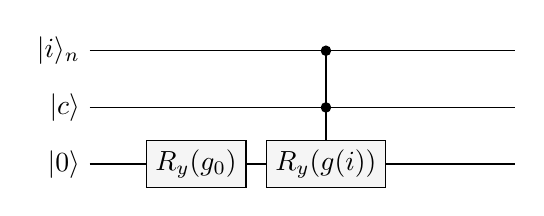
\begin{tikzpicture}[
        x=1cm,
        y=0.72cm,
        wire/.style={line width=0.5pt},
        dot/.style={circle, fill=black, inner sep=1.35pt},
        gate/.style={draw, fill=gray!8, minimum width=0.85cm, minimum height=0.55cm, align=center}
    ]
        \foreach \y/\lab in {2/{\lvert i\rangle_n},1/{\lvert c\rangle},0/{\lvert 0\rangle}}{
            \draw[wire] (0,\y) -- (5.4,\y);
            \node[left] at (0,\y) {$\lab$};
        }
        \node[gate] at (1.35,0) {$R_y(g_0)$};
        \node[dot] at (3.0,2) {};
        \node[dot] at (3.0,1) {};
        \draw[wire] (3.0,2) -- (3.0,0);
        \node[gate, minimum width=1.05cm] at (3.0,0) {$R_y(g(i))$};
    \end{tikzpicture}
    \caption{Payoff-loading rotation for the European call.  The comparator qubit $\lvert c\rangle$ activates the $i$-dependent rotation only on the branch $i\ge K$.}
    \label{fig:payoff-rotation-circuit}
\end{figure}

The Asian case uses the components at a greater cost.  Instead of loading a single terminal price, the circuit must prepare $N$ correlated monitoring-date prices, compute their arithmetic average into a work register using reversible adders, apply the comparator and payoff rotation to the average, and then uncompute the work registers so that $A^\dagger$ in Eq.~\eqref{eq:grover-iterate} returns the ancillas to a clean state.  Every Grover query therefore contains path loading, reversible averaging, comparison with the strike, payoff rotation, and the corresponding inverse operations.  This overhead is the circuit cost of path dependence, and it is why path-dependent options are often used to motivate quantum advantage in derivative pricing \cite{stamatopoulosOptionPricingUsing2020,wangOptionPricingStochastic2024}. There is a hitch, variance reduction, optimized integrators, and better sampling can make the practical gap much smaller than a simple-Monte-Carlo comparison suggests.

\section{Results and discussion}

\subsection{Classical benchmark}

The European call is mainly a check on the simulation pipeline.  Simple Monte Carlo converges to the Black--Scholes price with the expected $M^{-1/2}$ rate from Eq.~\eqref{eq:mc-se}.  With $5\times 10^5$ paths, averaged over $50$ independent trials, the mean standard error is $0.02081$ and the mean absolute error is $0.01456$.  This result is not computationally interesting by itself because the European call has a closed form.

The Asian option is the relevant classical benchmark.  Fig.~\ref{fig:asian-comparison} shows that the Kemna--Vorst control variate preserves the Monte Carlo exponent but changes the prefactor sharply.  At $M=100{,}000$ paths, the standard error falls from $0.025301$ for simple Monte Carlo to $0.000697$ with the control variate.  This is a standard-error reduction of $36.3$ and a variance reduction of $1.32\times 10^3$, consistent with the high correlation between arithmetic and geometric Asian payoffs used by Kemna and Vorst \cite{kemnaPricingMethodOptions1990,glassermanMonteCarloMethods2004}.

\begin{table}[H]
    \centering
    \caption{Benchmark checks for the Asian-pricing code.  Xu--Zhang--Wang values are from Table~4, row ``w/o ALL'', their plain Black--Scholes Monte Carlo ablation \cite{xuPricingArithmeticAverage2023}.}
    \label{tab:asian-benchmark-checks}
    \begin{tabular}{lccc}
        \toprule
        Check & Reference value & Our estimate & Diagnostic \\
        \midrule
        Geometric Asian & $5.565509$ & $5.577325\pm0.014132$ & $z=0.84$ \\
        Xu $T=30$ days  & $1.3871\pm0.0201$ & $1.4331\pm0.0020$ & $z=2.29$ \\
        Xu $T=90$ days  & $2.6589\pm0.0373$ & $2.7030\pm0.0038$ & $z=1.18$ \\
        Xu $T=180$ days & $4.0166\pm0.0546$ & $4.0870\pm0.0056$ & $z=1.29$ \\
        \bottomrule
    \end{tabular}
\end{table}

These checks have a narrow purpose.  They verify the simulation and control-variate implementation. They do not speak to the legitimacy of the market model as a predictor. For the Xu--Zhang--Wang rows, the diagnostic uses the Monte Carlo standard error reported in their table.  The $30$-day check is the loosest row, but it remains inside the three-standard-error band.  The quantum method is therefore being measured against a validated variance-reduced baseline, not only against simple Monte Carlo.

\subsection{European quantum validation}

The European call has a closed form, which makes it useful as a calibration problem.  The statevector calculation removes sampling noise and IAE uncertainty, so the test isolates the pricing map in Eqs.~\eqref{eq:distribution-loading}--\eqref{eq:amplitude-expectation}.  If the state preparation and payoff rotation are correct, the objective-qubit probability should reproduce the Black--Scholes price after the known rescaling in Eq.~\eqref{eq:european-amplitude-price}.

\begin{figure}[H]
    \centering
    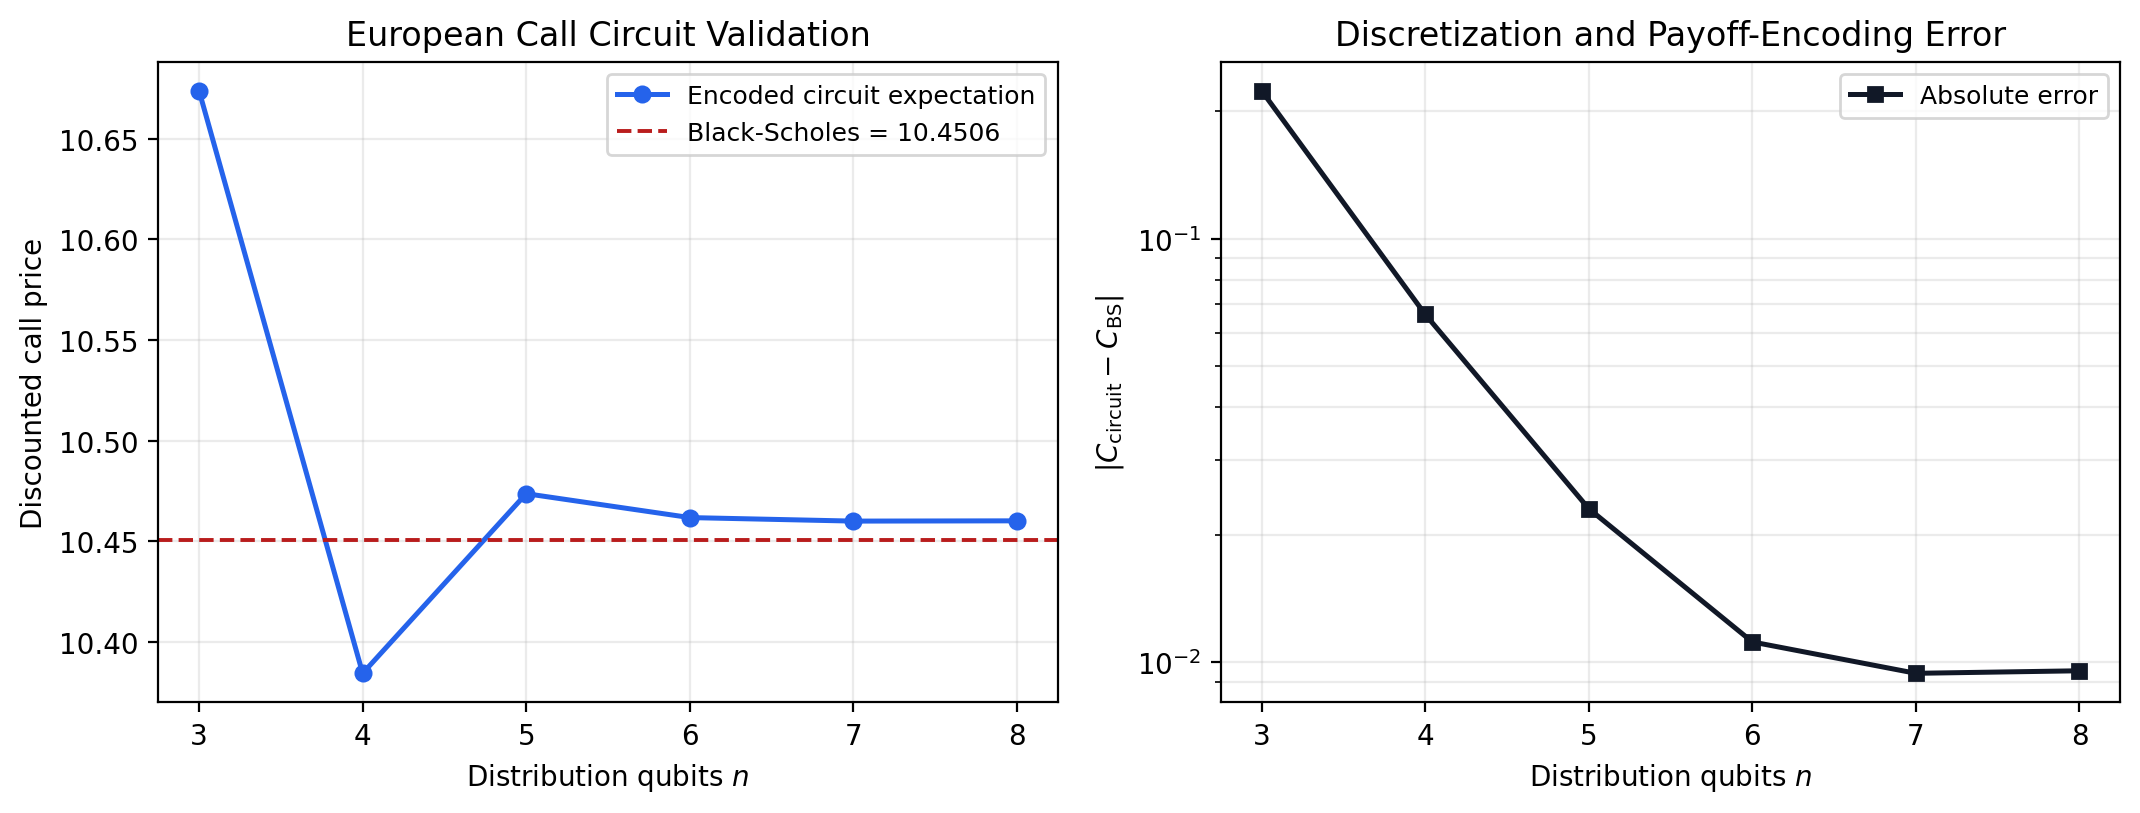
\includegraphics[width=0.82\textwidth]{quantum_european_statevector_convergence.png}
    \caption{European-call circuit validation using exact statevector probabilities.  The comparison tests the encoded amplitude, not the sampling behavior of IAE.}
    \label{fig:european-quantum-validation}
\end{figure}

The encoded price is already close with a small register.  At $n=3$ distribution qubits the circuit gives $10.673862$, an absolute error of $0.223279$ against the Black--Scholes price $10.450584$.  At $n=6$ the error falls to $0.011167$.  It then plateaus near $10^{-2}$, with errors $0.009416$ and $0.009547$ at $n=7$ and $n=8$. It seems like refining the price grid helps up to a limit.

IAE estimates the amplitude already present in the circuit \cite{grinkoIterativeQuantumAmplitude2021}.  It does not remove truncation error in the log-normal grid, nor does it repair the first-order payoff rotation used in the Stamatopoulos construction \cite{stamatopoulosOptionPricingUsing2020}.  The statevector result therefore validates the circuit as an amplitude-encoding implementation, but not as a hardware speedup.

\subsection{Resource tradeoff}

The query speedup from QAE is meaningful only after the cost of one query is fixed.  Table~\ref{tab:european-resources} reports the compiled size of the European $A$ operator.  One Grover iterate contains $A$, $A^\dagger$, and two reflections, so an IAE run repeats a circuit at least of this scale many times.  The counts are generated by \texttt{scripts/generate\_quantum\_results.py --quick} with Qiskit~2.3.1, Qiskit Finance~0.4.1, and Qiskit Algorithms~0.4.0, transpiled to the \texttt{cx,u} basis at optimization level~$1$.  Grinko \textit{et al.}\ reduce the estimation overhead by avoiding QPE, but the state-preparation and payoff oracles remain the dominant problem-specific cost \cite{grinkoIterativeQuantumAmplitude2021}.

\begin{table}[H]
    \centering
    \caption{Transpiled European-call $A$-operator resources.  Counts are for state preparation and payoff loading only.}
    \label{tab:european-resources}
    \begin{tabular}{ccccc}
        \toprule
        Distribution qubits & Grid points & Total qubits & Depth & CX gates \\
        \midrule
        $3$ & $8$   & $7$  & $143$ & $94$  \\
        $4$ & $16$  & $9$  & $218$ & $141$ \\
        $5$ & $32$  & $11$ & $303$ & $196$ \\
        $6$ & $64$  & $13$ & $426$ & $267$ \\
        $7$ & $128$ & $15$ & $607$ & $370$ \\
        $8$ & $256$ & $17$ & $922$ & $537$ \\
        \bottomrule
    \end{tabular}
\end{table}

\begin{table}[H]
    \centering
    \caption{Toy arithmetic-Asian oracle checks.  Each monitoring date uses a two-qubit shock grid.  These circuits validate the finite-grid payoff map; they are not production resource estimates.}
    \label{tab:asian-toy-resources}
    \begin{tabular}{ccccc}
        \toprule
        Monitoring dates & Grid paths & Total qubits & Depth & CX gates \\
        \midrule
        $2$ & $16$ & $5$ & $293$  & $194$  \\
        $3$ & $64$ & $7$ & $2396$ & $1963$ \\
        \bottomrule
    \end{tabular}
\end{table}

The growth is moderate for the European call because the payoff depends only on $S_T$, unlike the Asian circuit.  Table~\ref{tab:asian-toy-resources} shows the same payoff map on small finite grids.  The three-date circuit reproduces its exact grid price to numerical precision, but it already reaches depth $2396$ before amplitude estimation.  A linear extrapolation from three dates to $252$ dates would give depth on the order of $2\times10^5$ and about $1.6\times10^5$ CX gates before any Grover repetitions.  This estimate is only a scale check.  Exact finite-grid loading would grow faster, while a serious production oracle would need more structure than the toy circuit uses to compensate for market complicated market dynamics.

For the daily Asian option used in the classical benchmark, a quantum oracle would need to load $252$ correlated prices, compute the arithmetic average reversibly, compare it with the strike, rotate the payoff qubit, and uncompute the work registers.  Stamatopoulos \textit{et al.}\ identify this path-dependent structure as the place where reducing the number of samples could matter most \cite{stamatopoulosOptionPricingUsing2020}.  Wang and Kan reach a similar conclusion under stochastic volatility, where the resource analysis is dominated by arithmetic and path simulation circuits rather than by the abstract QAE primitive \cite{wangOptionPricingStochastic2024}.

These counts are still noiseless circuit counts.  Stamatopoulos \textit{et al.}\ ran only small European-call instances on IBM hardware and needed error mitigation to reduce two-qubit gate errors \cite{stamatopoulosOptionPricingUsing2020}.  IAE removes the QFT register and deep controlled powers, but it still requires repeated coherent applications of the Grover algorithm \cite{grinkoIterativeQuantumAmplitude2021}.  For larger path-dependent contracts, the relevant hardware question is therefore not only the number of oracle calls, but whether the full oracle can be executed with enough fidelity.  This is why fault-tolerant resource estimates, such as the $T$-count and $T$-depth analysis in Wang and Kan, are more informative than query counts alone \cite{wangOptionPricingStochastic2024}.

\section{Conclusion}

We studied option pricing with QAE against a variance-reduced classical baseline.  For the European call, the statevector calculation verifies the amplitude map used in the previous section.  After loading the log-normal terminal distribution and encoding the payoff into the objective qubit, the recovered price approaches the Black--Scholes value as the grid is refined.  The remaining error likely comes from grid truncation and payoff encoding.

The Asian option gives the more useful test.  With daily monitoring, the Kemna--Vorst control variate lowers the variance of the arithmetic Asian estimator by $1.32\times10^3$ at $10^5$ paths.  This changes the baseline by three orders of magnitude in variance.  On the quantum side, each Asian oracle must prepare the path distribution, compute the average reversibly, compare with the strike, load the payoff, and uncompute the work registers before the Grover iterate can be applied.
  The "quantum advantage" depends on the payoff, the available variance reduction, and the cost of implementing the oracle.  It also depends on hardware.  A deep oracle repeated inside amplitude estimation is sensitive to noise on present devices and expensive under error correction.  For the Black--Scholes Asian case considered here, the evidence points in one direction.  The query speedup is real, but it is not the bottleneck.  The bottleneck is the full path-dependent oracle, measured against a control variate that already removes most of the classical variance.

\printbibliography

\end{document}
